\documentclass{article}
\usepackage{amsmath}
\usepackage{tikz}

\begin{document}

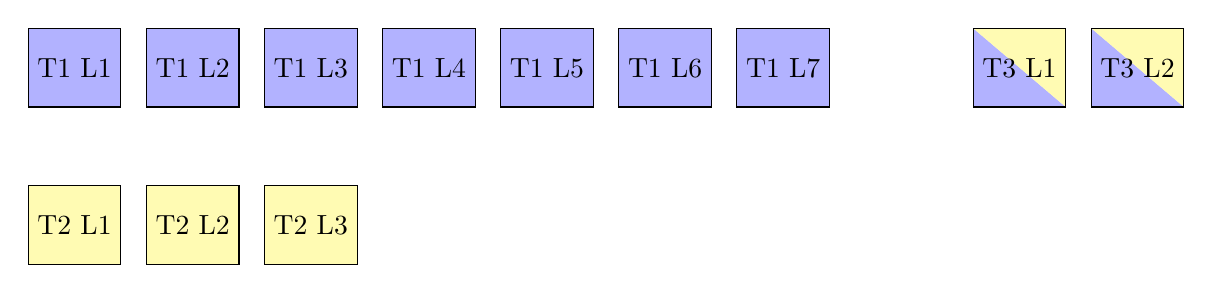
\begin{tikzpicture}
% Define styles
\tikzset{
    box/.style={draw, , minimum height=1cm, text centered},
    double color/.style={draw, minimum height=1cm, text centered, 
    fill=none, path picture={
      \fill[blue!30] (path picture bounding box.south west) -- (path picture bounding box.north west) -- (path picture bounding box.south east) -- cycle;
      \fill[yellow!30] (path picture bounding box.south east) -- (path picture bounding box.north west) -- (path picture bounding box.north east) -- cycle;
    }}
}
\node[box, fill=blue!30] (Box1) at (0,0) {T1 L1};
\node[box, fill=blue!30] (Box2) at (1.5,0) {T1 L2};
\node[box, fill=blue!30] (Box3) at (3,0) {T1 L3};
\node[box, fill=blue!30] (Box4) at (4.5,0) {T1 L4};
\node[box, fill=blue!30] (Box5) at (6,0) {T1 L5};
\node[box, fill=blue!30] (Box6) at (7.5,0) {T1 L6};
\node[box, fill=blue!30] (Box7) at (9,0) {T1 L7};

\node[box, fill=yellow!30] (Box8) at (0.0,-2) {T2 L1};
\node[box, fill=yellow!30] (Box9) at (1.5,-2) {T2 L2};
\node[box, fill=yellow!30] (Box10) at (3,-2) {T2 L3};
\node[double color] (Box11) at (12,0) {T3 L1};
\node[double color] (Box12) at (13.5,0) {T3 L2};
\end{tikzpicture}

\end{document}